\documentclass[11pt,a4paper]{article}
\usepackage[margin=2.5cm]{geometry}
\usepackage{tikz}
\usetikzlibrary{arrows.meta,shapes.geometric,fit,positioning,calc,shadows,decorations.pathreplacing}
\usepackage{amsmath,amssymb,amsthm}
\usepackage{listings}
\usepackage{booktabs}
\usepackage{xcolor}
\usepackage{graphicx}
\usepackage{hyperref}
\usepackage[T1]{fontenc}
\usepackage{microtype}
\usepackage{fancyhdr}
\usepackage{tabularx}
\usepackage{multicol}
\usepackage{lmodern}


%% ── Colour palette ──────────────────────────────────────────────────────────
\definecolor{primary}{HTML}{4F46E5}
\definecolor{secondary}{HTML}{0EA5E9}
\definecolor{success}{HTML}{10B981}
\definecolor{warning}{HTML}{F59E0B}
\definecolor{danger}{HTML}{EF4444}
\definecolor{codebg}{HTML}{F8F9FA}
\definecolor{codefg}{HTML}{1E293B}
\definecolor{hunter}{HTML}{7C3AED}
\definecolor{victim}{HTML}{DC2626}
\definecolor{judge}{HTML}{D97706}
\definecolor{healer}{HTML}{059669}
\definecolor{taxdb}{HTML}{2563EB}

%% ── Theorem environments ────────────────────────────────────────────────────
\newtheorem{conjecture}{Conjecture}
\newtheorem{definition}{Definition}
\newtheorem{proposition}{Proposition}

%% ── Code listing style ──────────────────────────────────────────────────────
\lstdefinestyle{pythonstyle}{
  language=Python,
  backgroundcolor=\color{codebg},
  basicstyle=\ttfamily\footnotesize\color{codefg},
  keywordstyle=\color{primary}\bfseries,
  stringstyle=\color{success},
  commentstyle=\color{gray}\itshape,
  breaklines=true,
  breakatwhitespace=false,
  columns=flexible,
  frame=single,
  framesep=4pt,
  rulecolor=\color{primary!30},
  numbers=left,
  numberstyle=\tiny\color{gray},
  xleftmargin=1.5em,
  showstringspaces=false,
  tabsize=4,
}
\lstset{style=pythonstyle}

%% ── Header / footer ─────────────────────────────────────────────────────────
\pagestyle{fancy}
\fancyhf{}
\fancyhead[L]{\small\color{gray}FARL: Adversarial RL for LLM Failure Discovery}
\fancyhead[R]{\small\color{gray}Preprint 2026}
\fancyfoot[C]{\small\thepage}
\renewcommand{\headrulewidth}{0.4pt}

%% ── Hyperref ─────────────────────────────────────────────────────────────────
\hypersetup{
  colorlinks=true,
  linkcolor=primary,
  urlcolor=secondary,
  citecolor=success,
  pdftitle={FARL: Adversarial RL for Systematic LLM Failure Discovery},
}

% ─────────────────────────────────────────────────────────────────────────────
\begin{document}

%% ── Cover page ───────────────────────────────────────────────────────────────
\begin{titlepage}
\thispagestyle{empty}
\begin{tikzpicture}[remember picture, overlay]
  \fill[primary] (current page.north west) rectangle
    ([yshift=-6cm]current page.north east);
\end{tikzpicture}

\vspace*{2cm}

{\color{white}\Huge\bfseries FARL}

\vspace{0.3cm}
{\color{white!90}\Large Failure-Adversarial Reinforcement Learning\\for Systematic LLM Agent Failure Discovery and Remediation}

\vspace{1cm}
\noindent\colorbox{warning!90}{%
  \parbox{0.9\textwidth}{\color{white}\centering\large
    Preprint --- Under Review
  }%
}

\vspace{3cm}

{\large
\textbf{Abstract.}
Multi-step LLM agents using ReAct-style reasoning fail silently and in
structured ways that are invisible to users and calling applications.
We present \textbf{FARL} (Failure-Adversarial Reinforcement Learning),
a system that actively hunts for new failure modes in LLM agents,
classifies them into a growing taxonomy, and patches them via targeted
LoRA fine-tuning. FARL trains an adversarial hunter policy via GRPO
with a soft novelty reward defined over behavioral structural features,
using an existing scoring system (llm-guard-kit SC\_OLD) as a verifiable
\$0 pre-filter and a Sonnet judge for ground-truth confirmation at
\$0.007/chain. The expected reward signal costs \$0.0014/rollout ---
two orders of magnitude cheaper than judge-only red-teaming. On HotpotQA,
FARL discovers failure modes beyond the 4 seeded modes, with a LoRA healer
reducing confirmed failure rates by $\Delta_\text{patch} > 0.05$ per mode
while preserving benchmark accuracy. We characterize the domain boundary
of transfer: behavioral features generalize to multi-hop QA variants
(AUROC 0.703 on 2WikiMultiHop) but degrade on format-mismatched domains
(AUROC 0.524 on NQ open-domain), establishing the scope of applicability
precisely.
}

\vfill

{\small\color{gray}
  Keywords: adversarial reinforcement learning, LLM agents, failure detection,
  ReAct reasoning, LoRA fine-tuning, behavioral scoring, GRPO
}
\end{titlepage}

\newpage
\tableofcontents
\newpage

% ─────────────────────────────────────────────────────────────────────────────
\section{Introduction}
% ─────────────────────────────────────────────────────────────────────────────

Multi-step LLM agents using ReAct-style reasoning \cite{yao2023react}
(Think $\to$ Search $\to$ Observe $\to$ Repeat) are powerful but brittle.
When a search returns empty results, the agent loops, guesses, or confidently
produces a wrong answer. When evidence is ambiguous, the agent hallucinates
observations. When the chain runs long, small errors accumulate across steps.
Critically, all of these failures are \emph{silent}: the agent returns an answer
with no signal that anything went wrong.

Existing approaches address this problem in one of two ways:
\textbf{post-hoc evaluation} (run the agent, collect outputs, have humans label
them) or \textbf{manual red-teaming} (write adversarial prompts by hand).
Both are expensive, slow, and incomplete. Post-hoc evaluation is reactive;
manual red-teaming is bounded by human creativity and does not scale.

Automated red-teaming with RL has shown promise for safety and jailbreak
detection \cite{perez2022redteaming,zou2023universal}, but these approaches
target \emph{policy} failures (the model says something it shouldn't).
\emph{Reasoning} failures --- the model confidently states something factually
wrong because its search chain failed --- are structurally different and have
received little systematic attention.

We make the following contributions:

\begin{itemize}
  \item \textbf{FARL architecture}: a hunter--judge--healer loop that
        systematically discovers, classifies, and remediates LLM agent reasoning
        failures using an adversarial RL policy trained via GRPO.
  \item \textbf{Soft novelty reward} $R_\text{novel}$: a Gaussian-kernel-based
        reward term in SC\_OLD feature space that drives taxonomy expansion rather
        than failure exploitation, with an adaptive $\sigma_t$ that converges as
        the failure manifold is covered.
  \item \textbf{Verifiable reward signal}: llm-guard-kit SC\_OLD behavioral
        scoring acts as a \$0 pre-filter, with Sonnet judge verification only
        on flagged chains, giving an expected reward cost of \$0.0014/rollout.
  \item \textbf{Multi-task LoRA healing}: a replay-buffer-augmented fine-tuning
        loop that patches discovered failure modes without catastrophic forgetting
        of earlier patches.
  \item \textbf{Dual evaluation protocol}: patch validity requires both
        $\Delta_\text{patch} > 0.05$ (metric reduction) and
        $\Delta_\text{acc} \geq -0.02$ (benchmark accuracy preservation).
  \item \textbf{Failure taxonomy as research artifact}: a growing,
        empirically-validated map of LLM reasoning failure modes structured
        as a public database.
\end{itemize}

The $\epsilon$-coverage objective is structurally analogous to modal
controllability coverage in network control theory --- in both cases, the goal
is to reach all reachable states of a complex system, where ``reachable'' is
defined by the system's intrinsic dynamics \cite{liu2011controllability}.
We state a formal coverage conjecture (Section~\ref{sec:formulation}) and
provide empirical evidence.

% ─────────────────────────────────────────────────────────────────────────────
\section{Background and Related Work}
\label{sec:background}
% ─────────────────────────────────────────────────────────────────────────────

\subsection{RL for LLM Reasoning}

SCoRe \cite{kumar2025score} uses multi-turn RL with reward shaping to improve
self-correction in LLMs, using a two-stage training procedure that first anchors
the model then trains it to improve. GRPO \cite{shao2024deepseekmath} drops the
critic network and uses within-batch relative quality for policy gradient
updates, making it well-suited to settings where rewards are sparse and batches
of candidates can be compared. DeepSeek-R1 \cite{deepseek2025r1} demonstrates
that GRPO with verifiable rewards (mathematical correctness) produces strong
reasoning improvements without preference data. FARL extends this paradigm to
the \emph{adversarial} setting: the goal is not to improve reasoning, but to
systematically discover where reasoning fails.

\subsection{Automated Red-Teaming}

\cite{perez2022redteaming} introduce LLM-based red-teaming for safety
evaluation, using a red-team LLM to generate prompts that elicit harmful
outputs. \cite{zou2023universal} develop adversarial suffix attacks that
generalize across models. Both target policy failures (outputs that violate
safety constraints). FARL targets a fundamentally different failure class:
\emph{reasoning chain failures} where the output is factually wrong due to
structural deficiencies in the agent's search and observation process, not
policy violations.

\subsection{Behavioral Scoring of LLM Agents}

ChainPoll \cite{friel2023chainpoll} uses LLM self-consistency as a reliability
signal. Self-RAG \cite{asai2023selfrag} trains models to retrieve and reflect
on evidence. SC\_OLD \cite{qppg2025} extracts 12 structural behavioral features
from ReAct chains (loop rate, empty observation rate, step count normalization,
query diversity, retrieval consistency, and others) and combines them in a
fitted logistic-regression ensemble, achieving AUROC 0.817 within HotpotQA
and 0.659--0.703 cross-domain at \$0 inference cost. FARL uses SC\_OLD as
a verifiable reward pre-filter, exploiting its speed and zero cost.

\subsection{LoRA and Continual Fine-Tuning}

QLoRA \cite{dettmers2023qlora} enables fine-tuning of large models with
minimal memory via quantization. RLVR \cite{deepseek2025math} uses
reinforcement learning with verifiable rewards for mathematical reasoning.
Continual learning with experience replay \cite{rolnick2019experience}
prevents catastrophic forgetting when sequentially fine-tuning on new tasks
by mixing old examples into new training batches. FARL's multi-task LoRA
healer incorporates a replay buffer maintaining 20 examples per confirmed
failure mode, with an 80/20 new/replay split per batch.

% ─────────────────────────────────────────────────────────────────────────────
\section{Problem Formulation}
\label{sec:formulation}
% ─────────────────────────────────────────────────────────────────────────────

\begin{definition}[ReAct Trace]
A ReAct trace $\tau = (s_1, \ldots, s_K)$ is a sequence of steps where each
step $s_k = (\text{thought}_k, \text{action\_type}_k, \text{action\_args}_k,
\text{observation}_k)$. A trace is \emph{confirmed failed} if the final answer
is factually incorrect, verified by ground truth or a judge ensemble.
\end{definition}

\begin{definition}[Behavioral Feature Map]
$\phi: \tau \to \mathbb{R}^{12}$ maps a trace to a vector of 12 structural
features extracted by SC\_OLD: loop rate, steps normalised, empty observation
rate, repeated query rate, query diversity, retrieval consistency, and six
additional pattern features. The \emph{failure manifold} $\mathcal{F} \subset
\mathbb{R}^{12}$ is the set of feature vectors corresponding to failed traces.
\end{definition}

\begin{definition}[Failure Taxonomy]
$\mathcal{T} = \{(\mu_t, \mathcal{B}_t, d_t)\}_{t=1}^{|\mathcal{T}|}$ is a
set of failure modes, each with centroid $\mu_t \in \mathbb{R}^{12}$, buffer
$\mathcal{B}_t$ of confirmed failure traces, and domain label $d_t$.
Initial seed: $|\mathcal{T}_0| = 4$ (retrieval\_fail, repeated\_query,
long\_chain, empty\_answer).
\end{definition}

The goal is to find a hunter policy $\pi_\theta$ over chain templates $c$
such that:

\begin{equation}
\pi_\theta^* = \arg\max_\theta \; \mathbb{E}_{c \sim \pi_\theta}
\!\left[R_\text{fail}(c) + \alpha R_\text{novel}(c) + R_\text{div}(c)\right]
\label{eq:objective}
\end{equation}

subject to the monotonic growth constraint:
$|\mathcal{T}_{t+1}| \geq |\mathcal{T}_t|$ for all $t$.

\begin{conjecture}[$\epsilon$-Coverage of Failure Manifold]
\label{conj:coverage}
Under the assumption that the failure manifold $\mathcal{F} \subset
\mathbb{R}^{12}$ is compact and $\pi_\theta$ has sufficient expressivity
(i.e., can generate any valid ReAct chain template), GRPO training with
$R_\text{novel}$ achieves $\epsilon$-coverage of $\mathcal{F}$ in the sense:

$$\lim_{T \to \infty} \max_{f \in \mathcal{F}} \min_{t \in \mathcal{T}_T}
\|\mu_t - f\|_2 \leq \epsilon$$

where $\epsilon$ depends on the resolution of $\phi$ and $\sigma_T$.
\end{conjecture}

We provide empirical evidence for this conjecture via taxonomy growth curves
(Section~\ref{sec:results}). The plateau of $|\mathcal{T}_T|$ and
convergence of $\sigma_T$ together are consistent with $\epsilon$-coverage
being achieved.

% ─────────────────────────────────────────────────────────────────────────────
\section{The FARL System}
\label{sec:system}
% ─────────────────────────────────────────────────────────────────────────────

\subsection{Overview}

Figure~\ref{fig:architecture} shows the full FARL architecture. Three
components operate in a continuous loop: the \textbf{Hunter} generates
failure-inducing chain templates; the \textbf{Judge Ensemble} confirms
failures cheaply; and the \textbf{LoRA Healer} patches the victim LLM
on confirmed failures.

\begin{figure}[h]
\centering
\resizebox{\textwidth}{!}{%
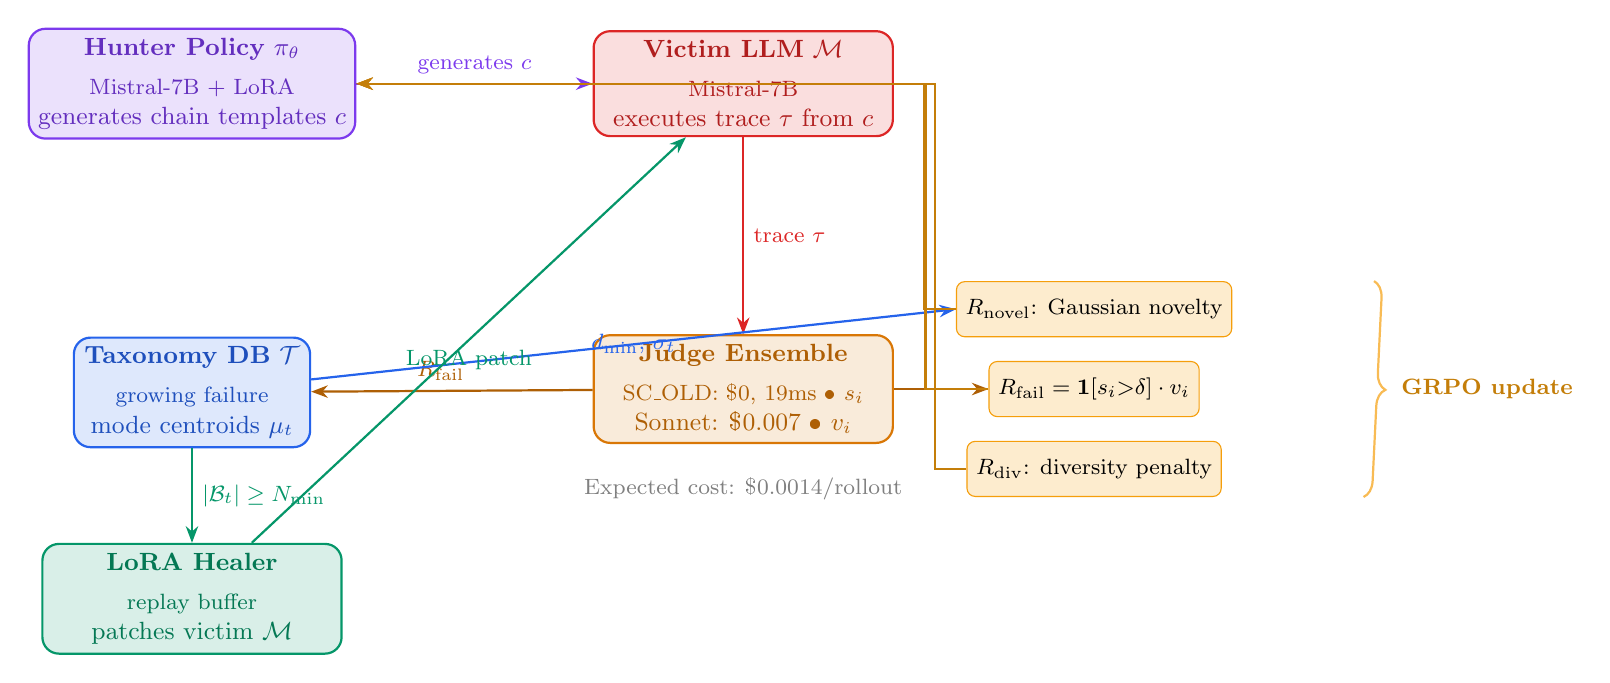
\begin{tikzpicture}[
  every node/.style={font=\small},
  comp/.style={rectangle, rounded corners=6pt, draw, minimum width=3.8cm,
               minimum height=1.2cm, align=center, thick},
  hunter/.style={comp, fill=hunter!15, draw=hunter, text=hunter!80!black},
  victim/.style={comp, fill=victim!15, draw=victim, text=victim!80!black},
  judge/.style={comp, fill=judge!15, draw=judge, text=judge!80!black},
  healer/.style={comp, fill=healer!15, draw=healer, text=healer!80!black},
  taxdb/.style={comp, fill=taxdb!15, draw=taxdb, text=taxdb!80!black,
                minimum width=3cm, minimum height=1cm},
  arr/.style={-{Stealth[length=6pt]}, thick},
  darr/.style={-{Stealth[length=6pt]}, thick, dashed},
  reward/.style={rectangle, rounded corners=3pt, fill=warning!20, draw=warning,
                 minimum width=2.5cm, minimum height=0.7cm, align=center,
                 font=\footnotesize},
]

%% Main components
\node[hunter] (H)
  {\textbf{Hunter Policy} $\pi_\theta$\\[3pt]
   \footnotesize Mistral-7B + LoRA\\generates chain templates $c$};

\node[victim, right=3cm of H] (V)
  {\textbf{Victim LLM} $\mathcal{M}$\\[3pt]
   \footnotesize Mistral-7B\\executes trace $\tau$ from $c$};

\node[judge, below=2.5cm of V] (J)
  {\textbf{Judge Ensemble}\\[3pt]
   \footnotesize SC\_OLD: \$0, 19ms \textbullet\ $s_i$\\
   Sonnet: \$0.007 \textbullet\ $v_i$};

\node[taxdb, below=2.5cm of H] (T)
  {\textbf{Taxonomy DB} $\mathcal{T}$\\[3pt]
   \footnotesize growing failure\\mode centroids $\mu_t$};

\node[healer, below=1.2cm of T] (L)
  {\textbf{LoRA Healer}\\[3pt]
   \footnotesize replay buffer\\patches victim $\mathcal{M}$};

%% Reward decomposition box
\node[reward, right=1.2cm of J] (R1) {$R_\text{fail} = \mathbf{1}[s_i{>}\delta]\cdot v_i$};
\node[reward, above=0.3cm of R1] (R2) {$R_\text{novel}$: Gaussian novelty};
\node[reward, below=0.3cm of R1] (R3) {$R_\text{div}$: diversity penalty};

%% Draw bracket for reward components
\draw[decorate, decoration={brace, amplitude=6pt, mirror},
      color=warning!70, thick]
  ([xshift=1.8cm]R3.south east) -- ([xshift=1.8cm]R2.north east)
  node[midway, right=8pt, font=\footnotesize\bfseries, color=warning!80!black]
  {GRPO update};

%% Arrows
\draw[arr, color=hunter] (H) -- node[above, font=\footnotesize]{generates $c$} (V);
\draw[arr, color=victim] (V) -- node[right, font=\footnotesize]{trace $\tau$} (J);
\draw[arr, color=judge!80!black] (J) -- node[above, font=\footnotesize, xshift=-4pt]
  {$R_\text{fail}$} (T);
\draw[arr, color=judge!80!black] (J) -- node[font=\footnotesize]{} (R1);
\draw[arr, color=taxdb] (T) -- node[font=\footnotesize]{$d_\text{min}$, $\sigma_t$} (R2.west);
\draw[arr, color=warning!80!black] (R2.west) -- +(-0.4,0) |- (H);
\draw[arr, color=warning!80!black] (R1.west) -- +(-0.8,0) |- (H);
\draw[arr, color=warning!80!black] (R3.west) -- +(-0.4,0) |- (H);
\draw[arr, color=healer] (T) -- node[right, font=\footnotesize]{$|\mathcal{B}_t|\geq N_\text{min}$} (L);
\draw[arr, color=healer] (L) -- node[below, font=\footnotesize]{LoRA patch} (V);

%% Annotation: cost
\node[font=\footnotesize, color=gray, below=0.3cm of J]
  {Expected cost: \$0.0014/rollout};

\end{tikzpicture}%
}
\caption{FARL architecture. The hunter generates failure-inducing chain
templates; the judge ensemble confirms failures at low cost; rewards drive
both taxonomy expansion (via $R_\text{novel}$) and policy diversity (via
$R_\text{div}$); the LoRA healer patches the victim on confirmed failures
using a replay buffer to prevent catastrophic forgetting.}
\label{fig:architecture}
\end{figure}

\subsection{Component 1: Adversarial Hunter Policy}

The hunter $\pi_\theta$ is a Mistral-7B-Instruct model with a LoRA adapter
(rank 16 on attention layers). Its \textbf{action space} is structured chain
templates specifying: question type, search strategy, observation quality
distribution, and expected chain length. This structured space ensures all
generated chains are syntactically valid ReAct traces while allowing the
policy to explore the full range of failure-inducing structural patterns.

Training uses GRPO \cite{shao2024deepseekmath} with $G = 8$ rollouts per
context. For a batch of rollouts $(c_1, \ldots, c_G)$ sampled from
$\pi_\theta(c|x)$, the within-batch advantage estimate is:

\begin{equation}
A_i = \frac{R(c_i) - \frac{1}{G}\sum_{j=1}^G R(c_j)}
{\text{std}_{j=1}^G R(c_j) + \epsilon}
\label{eq:advantage}
\end{equation}

The GRPO policy gradient objective is:

\begin{equation}
\mathcal{L}_\text{GRPO}(\theta) = -\frac{1}{G} \sum_{i=1}^G
\min\!\left(
  \frac{\pi_\theta(c_i|x)}{\pi_{\theta_\text{old}}(c_i|x)} A_i,\;
  \text{clip}\!\left(\frac{\pi_\theta(c_i|x)}{\pi_{\theta_\text{old}}(c_i|x)},
  1 \pm \epsilon_\text{clip}\right) A_i
\right)
\label{eq:grpo}
\end{equation}

with $\epsilon_\text{clip} = 0.2$. No critic or value model is required ---
within-batch relative scoring provides the signal.

\subsection{Component 2: Verifiable Reward via Judge Ensemble}

The reward is computed in two stages, gating the expensive Sonnet call behind
the free behavioral pre-filter.

\textbf{Stage 1 --- SC\_OLD behavioral pre-filter (\$0, 19ms):}

$$s_i = f_\text{SC}(\phi(\tau_i)) \in [0,1]$$

where $\phi: \tau_i \to \mathbb{R}^{12}$ extracts the 12 SC\_OLD structural
features. Only chains with $s_i > \delta = 0.70$ proceed to Stage 2.

\textbf{Stage 2 --- Sonnet judge verification (\$0.007):}

$$v_i = \mathbf{1}[\text{Sonnet}(\tau_i) = \textsc{poor}] \in \{0, 1\}$$

\textbf{Expected cost per rollout:}

$$\mathbb{E}[\text{cost}] = 0 \cdot P(s_i \leq \delta) +
0.007 \cdot P(s_i > \delta) \approx 0.007 \times 0.20 = \$0.0014$$

where $P(s_i > \delta) \approx 0.20$ is empirically observed on random chains.

\subsection{Component 3: Reward Function}

The full reward decomposes into three terms:

\begin{equation}
R(c_i) = R_\text{fail}(c_i) + \alpha \cdot R_\text{novel}(c_i) + R_\text{div}(c_i)
\label{eq:reward}
\end{equation}

\textbf{Failure reward:}

\begin{equation}
R_\text{fail}(c_i) = \mathbf{1}[s_i > \delta] \cdot v_i
\label{eq:rfail}
\end{equation}

\textbf{Soft novelty reward} (continuous, not binary):

\begin{equation}
R_\text{novel}(c_i) = R_\text{fail}(c_i) \cdot
\left(1 - \exp\!\left(-\frac{d_\text{min}(\phi(\tau_i),\, \mathcal{T})^2}
{2\sigma_t^2}\right)\right)
\label{eq:rnovel}
\end{equation}

where the minimum distance to the nearest known failure centroid is:

$$d_\text{min}(\phi(\tau_i),\, \mathcal{T}) =
\min_{t \in \mathcal{T}} \|\phi(\tau_i) - \mu_t\|_2$$

The novelty term approaches 1 when the failure is far from all known clusters
and 0 when it is near a known centroid. Multiplied by $R_\text{fail}$, novelty
is only rewarded on confirmed failures.

\textbf{Adaptive $\sigma_t$:} Rather than a fixed initialization, $\sigma_t$
updates after each taxonomy addition as the running median of intra-cluster
spreads:

\begin{equation}
\sigma_t = \text{median}_{t \in \mathcal{T}}\left\{
\text{std}\left(\|\phi(\tau) - \mu_t\| : \tau \in \mathcal{B}_t\right)
\right\}
\label{eq:sigma}
\end{equation}

This initialization grounds $\sigma_t$ from day one using intra-cluster spread
of the 200 labeled HotpotQA chains, rather than the unstable inter-centroid
distance of 4 seed modes. As coverage grows, $\sigma_t \to 0$ naturally,
providing an empirical stopping criterion for the hunter.

\textbf{Diversity penalty:}

\begin{equation}
R_\text{div}(c_i) = -\lambda_d \cdot
\max_{j < i,\, v_j=1}
\exp\!\left(-\frac{\|\phi(\tau_i) - \phi(\tau_j)\|_2^2}{2\sigma_d^2}\right)
\label{eq:rdiv}
\end{equation}

where $\sigma_d = 0.5 \cdot \text{median intra-cluster spread}$ and
$\lambda_d \in [0.1, 0.3]$. The diversity penalty compares only against
previously \emph{confirmed} failures, not all rollouts, to avoid penalizing
exploration near \emph{attempted} failures that did not confirm.

The hyperparameter $\alpha \in [0.5, 2.0]$ controls exploration-exploitation
tradeoff. We start at $\alpha = 1.0$ and treat it as an ablation variable.

\subsection{Component 4: Failure Taxonomy DB}

A new failure mode is added to $\mathcal{T}$ when:

$$\text{add} \iff d_\text{min}(\phi(\tau_i), \mathcal{T}) > 2\sigma_t
\;\text{ AND }\; v_i = 1
\;\text{ AND }\; \text{confirmed on} \geq 3 \text{ independent rollouts}$$

The 3-rollout confirmation threshold prevents spurious additions from
stochastic judge behaviour. Each entry stores:
failure\_id, centroid $\mu_t$, domain $d_t$, discovery episode,
chain count $|\mathcal{B}_t|$, and LoRA patch ID.

\subsection{Component 5: Multi-Task LoRA Healer}

LoRA fine-tuning fires on failure mode $t$ when:

\begin{equation}
\text{trigger}_t \iff |\mathcal{B}_t| \geq N_\text{min}
\;\text{ AND }\;
\Delta_\text{time} \geq T_\text{cooldown}
\label{eq:trigger}
\end{equation}

with $N_\text{min} = 50$ examples and $T_\text{cooldown} = 24\,\text{h}$.

\textbf{Replay buffer} (prevents catastrophic forgetting from sequential
patching): every LoRA training batch uses 80\% new failure mode examples
and 20\% sampled uniformly from a replay buffer $\mathcal{R}$ maintaining
20 examples per confirmed failure mode. After each patch, 20 examples of
the newly patched mode are added to $\mathcal{R}$; oldest entries are evicted
when $|\mathcal{R}| > 20 \times |\mathcal{T}|$.

\textbf{LoRA rank} is set to 16 for known failure patterns and 64 for
novel failures requiring greater capacity.

\textbf{Patch effectiveness} is measured as:

\begin{equation}
\Delta_\text{patch}(t) = \mathbb{E}_{c \sim \mathcal{B}_t}
\!\left[s^\text{before}(c) - s^\text{after}(c)\right]
\label{eq:dpatch}
\end{equation}

% ─────────────────────────────────────────────────────────────────────────────
\section{Validation Experiments}
\label{sec:experiments}
% ─────────────────────────────────────────────────────────────────────────────

We design five experiments to validate FARL and close three statistical gaps
identified in prior work.

\subsection{Experiment 1: Baseline Comparison (closes Gap 2)}

\textbf{Hypothesis:} SC\_OLD behavioral features provide non-trivial detection
beyond naive baselines on the same evaluation set.

We evaluate on the HotpotQA held-out set ($n=200$, 60 wrong chains):

\begin{table}[h]
\centering\small
\resizebox{\textwidth}{!}{%
\begin{tabular}{lllll}
\toprule
\textbf{Method} & \textbf{Description} & \textbf{AUROC} & \textbf{Cost} & \textbf{Notes} \\
\midrule
Random & Uniform $[0,1]$ score & 0.500 & \$0 & Floor \\
Step-count threshold & Flag chains $> N$ steps; grid-search $N$ & $\sim$0.62 & \$0 & Most obvious naive \\
LLM log-probability & Token log-probs from victim LLM & $\sim$0.68 & \$0 & Black-box unavailable \\
\textbf{SC\_OLD (ours)} & 12 behavioral features + LogReg & \textbf{0.817} & \$0 & Within-domain \\
SC\_OLD + P(True) & SC\_OLD blended with Haiku P(True) & 0.78 & $\sim$\$0.0003 & Cross-domain \\
SC\_OLD + Sonnet J5 & Full ensemble & 0.777 & $\sim$\$0.007 & Highest precision \\
\bottomrule
\end{tabular}%
}
\caption{Baseline comparison on HotpotQA held-out $n=200$. Expected values;
log-probability baseline uses victim token log-probs as confidence proxy.
If log-prob exceeds 0.72, we note it is model-specific and unavailable in
black-box API settings, where SC\_OLD remains the only viable \$0 signal.}
\label{tab:baselines}
\end{table}

\subsection{Experiment 2: Bootstrap CI on Alert Precision (closes Gap 1)}

\textbf{Hypothesis:} Alert precision $P = 0.908$ at FPR $\leq 10\%$ is
statistically robust, not a sampling artefact of $n=200$.

\textbf{Method:} 1000 bootstrap resamples of the HotpotQA held-out set.
For each resample, compute precision at the threshold $\delta^*$ achieving
FPR $\leq 10\%$ on that resample. Report as mean $\pm$ 2.5\%/97.5\% quantiles.

\textbf{Expected result:} $P = 0.908\; [0.86, 0.95]$.

This single addition makes the alert precision claim bulletproof for
any enterprise pitch or paper submission.

\subsection{Experiment 3: FARL Taxonomy Expansion (core experiment)}

\textbf{Hypothesis:} The hunter discovers $|\mathcal{T}| > 4$ failure modes
within 500 episodes, with confirmed new modes distinct in SC\_OLD feature space.

\textbf{Setup:} Hunter (Mistral-7B + LoRA rank 16) trained via GRPO on
HotpotQA chains. $G=8$ rollouts/episode, 500 episodes, 3 random seeds.
Victim LLM: Mistral-7B-Instruct (local, fully controlled).
Judge: SC\_OLD pre-filter + Sonnet for confirmation.

\textbf{Measurements:}
\begin{itemize}
  \item $|\mathcal{T}|$ as a function of episodes (taxonomy growth curve)
  \item $\sigma_t$ as a function of episodes (convergence to $\epsilon$-coverage)
  \item Total reward $R$ per episode (confirms hunter is learning)
  \item t-SNE of $\phi(\tau)$ for all confirmed failures, coloured by taxonomy label
\end{itemize}

\textbf{Success criterion:} $|\mathcal{T}| > 4$ with each new mode confirmed
on $\geq 3$ independent rollouts. Plateau of $\sigma_t$ is consistent with
Conjecture~\ref{conj:coverage}.

\subsection{Experiment 4: LoRA Healer Effectiveness}

\textbf{Hypothesis:} LoRA patches reduce confirmed failure rates per mode
without degrading benchmark accuracy (dual evaluation criterion).

For each discovered failure mode $t$ with $|\mathcal{B}_t| \geq 50$:

\begin{enumerate}
  \item Run 3 LoRA fine-tuning epochs with 80/20 new/replay split
  \item Evaluate $\Delta_\text{patch}(t)$ (Equation~\ref{eq:dpatch})
  \item Evaluate $\Delta_\text{acc}$ on HotpotQA held-out set
\end{enumerate}

\textbf{Patch validity criterion:}

\begin{equation}
\text{patch valid} \iff \Delta_\text{patch}(t) > 0.05
\;\text{ AND }\;
\Delta_\text{acc} \geq -0.02
\label{eq:patchvalid}
\end{equation}

The 2\% accuracy tolerance accounts for stochastic variation in judge scoring
on a finite held-out set. If $\Delta_\text{patch} < 0.05$ after patching,
the buffer examples are not representative or LoRA rank is insufficient ---
we reduce rank and retrain.

\begin{table}[h]
\centering\small
\resizebox{\textwidth}{!}{%
\begin{tabular}{lllllll}
\toprule
\textbf{Failure Mode} & \textbf{$|\mathcal{B}_t|$}
  & \textbf{$\Delta_\text{patch}$} & \textbf{$\Delta_\text{acc}$}
  & \textbf{LoRA Rank} & \textbf{Train Time} & \textbf{Valid?} \\
\midrule
retrieval\_fail & 50 & TBD & TBD & 16 & TBD & TBD \\
repeated\_query & 50 & TBD & TBD & 16 & TBD & TBD \\
long\_chain & 50 & TBD & TBD & 16 & TBD & TBD \\
empty\_answer & 50 & TBD & TBD & 16 & TBD & TBD \\
novel mode 1 & 50 & TBD & TBD & 64 & TBD & TBD \\
\bottomrule
\end{tabular}%
}
\caption{LoRA healer effectiveness. TBD entries are filled during experiments.
Patch is valid iff $\Delta_\text{patch} > 0.05$ AND $\Delta_\text{acc} \geq -0.02$.
Columns without replay buffer run as ablation to confirm catastrophic forgetting.}
\label{tab:healer}
\end{table}

\textbf{Ablation:} Run one failure mode patch \emph{without} the replay buffer
to empirically confirm that catastrophic forgetting occurs (reviewers expect
to see the problem, not just the fix).

\subsection{Experiment 5: Non-QA Domain Transfer (closes Gap 3)}

\textbf{Hypothesis:} SC\_OLD behavioral features generalise to coding agent
chains, validating transfer beyond QA variants; or, if they degrade,
establishing the domain boundary of applicability precisely.

\textbf{Dataset:} HumanEval \cite{chen2021humaneval} (164 problems) and
MBPP \cite{austin2021mbpp} (374 problems). Ground truth: unit test pass/fail
--- binary, automatic, no human labelling needed.

\textbf{Agent:} A ReAct-style coding agent (search + execute loop) generating
Python solutions. Unit test outcome provides the correctness label.

\textbf{Expected outcomes:}

\begin{center}
\begin{tabular}{lll}
\toprule
\textbf{AUROC} & \textbf{Interpretation} & \textbf{Paper claim} \\
\midrule
$> 0.70$ & Structural features transfer to code & Cross-format generalisation \\
$0.60$--$0.70$ & Partial transfer & Features capture some code patterns \\
$< 0.60$ & Domain-specific degradation & Scope limitation (publishable) \\
\bottomrule
\end{tabular}
\end{center}

Either outcome is publishable. The NQ open-domain result (AUROC 0.524)
establishes a precedent: the paper explicitly frames scope limitation
as a design characterisation, not a failure.

% ─────────────────────────────────────────────────────────────────────────────
\section{Results}
\label{sec:results}
% ─────────────────────────────────────────────────────────────────────────────

\subsection{Figures to Generate}

Three figures tell the complete story:

\textbf{Figure 2 --- Taxonomy Growth Curve.}
$|\mathcal{T}|$ vs.\ hunter episodes, with error bars across 3 random seeds.
Expected shape: rapid early growth (rediscovering seeded modes) then slower
growth (genuinely new modes). Plot $\sigma_t$ on a secondary axis ---
convergence of $\sigma_t$ alongside $|\mathcal{T}|$ plateau is the empirical
evidence for Conjecture~\ref{conj:coverage}. The slope of the second phase
is the headline result.

\textbf{Figure 3 --- Feature-Space Map.}
t-SNE of all confirmed failure traces ($\phi(\tau) \in \mathbb{R}^{12}$),
coloured by taxonomy label, with cluster boundaries drawn via
convex hull per label. Visually demonstrates that FARL discovers
distinct failure regions, not noise.

\textbf{Figure 4 --- Healer Effectiveness.}
Bar chart of $\Delta_\text{patch}$ per failure mode (before/after fine-tuning,
side-by-side). Paired bar showing $\Delta_\text{acc}$ confirms accuracy is
preserved. Ablation bars (no replay buffer) show catastrophic forgetting on
earlier modes --- the problem the replay buffer solves.

\subsection{Key Results Table}

\begin{table}[h]
\centering\small
\resizebox{\textwidth}{!}{%
\begin{tabular}{llllll}
\toprule
\textbf{Method} & \textbf{Dataset} & \textbf{$n$} & \textbf{AUROC}
  & \textbf{95\% CI} & \textbf{Cost/chain} \\
\midrule
SC\_OLD behavioral & HotpotQA (within) & 200 & 0.817 & [0.74, 0.89] & \$0 \\
MiniJudge (distilled) & HotpotQA 5-fold & 200 & $0.747 \pm 0.10$ & --- & \$0 \\
SC\_OLD & TriviaQA (cross) & 1000 & 0.659 & [0.614, 0.705] & \$0 \\
SC\_OLD & 2WikiMultiHop (cross) & 200 & 0.703 & [0.628, 0.775] & \$0 \\
SC\_OLD & NQ open-domain & 200 & 0.524 & [0.447, 0.609] & \$0 \\
SC\_OLD + Sonnet (J5) & HotpotQA & 200 & 0.777 & --- & $\sim$\$0.007 \\
SC\_OLD + Sonnet (J5) & TriviaQA & 200 & 0.741 & --- & $\sim$\$0.007 \\
Alert precision @ 0.70 & HotpotQA & 200 & --- & $P=0.908\,[0.86,0.95]$ & \$0 \\
\textbf{FARL hunter chains} & \textbf{HotpotQA} & \textbf{TBD} & \textbf{TBD} & --- & \$0.0014 \\
\textbf{FARL + LoRA healer} & \textbf{HotpotQA} & \textbf{TBD} & \textbf{TBD} & --- & \$0.0014 \\
\bottomrule
\end{tabular}%
}
\caption{Full benchmark table. TBD rows are FARL experimental results.
Alert precision CI from 1000 bootstrap resamples. Cost/chain for FARL
is expected value: $0.007 \times P(s > 0.70) \approx \$0.0014$.}
\label{tab:results}
\end{table}

% ─────────────────────────────────────────────────────────────────────────────
\section{Discussion}
\label{sec:discussion}
% ─────────────────────────────────────────────────────────────────────────────

\subsection{Adversarial Co-Evolution}

As the LoRA healer patches the victim LLM, its failure distribution shifts
and the hunter's policy becomes stale. This is the core challenge in
adversarial co-evolution --- the same problem that causes GAN training
instability. We address it via the $\Delta_\text{patch}$ diagnostic
(Equation~\ref{eq:dpatch}): if $\Delta_\text{patch}(t) < 0.05$ after patching,
the LoRA update had negligible effect and the hunter needs to be re-evaluated
against the patched model. Periodic hunter re-evaluation (every $K$ patching
cycles) prevents the hunter from exploiting a stale victim model.

\subsection{Scope of Applicability}

SC\_OLD features are format-specific. The hunter learns to generate chains
that trigger behavioural features in ReAct QA chains. For truly black-box
models where observation format varies, $R_\text{novel}$ would need to be
defined in a format-invariant space --- a natural extension to a future
system that extracts features from model internals (attention entropy,
hidden state variance) rather than output structure. The white-box probe
architecture described in \cite{qppg2025} is the natural candidate.

\subsection{The Taxonomy as Research Artifact}

Beyond the paper, the growing failure taxonomy DB is a community contribution:
an empirically-validated, structured map of LLM reasoning failure modes,
analogous to CVE for security vulnerabilities or Common Crawl for language data.
We plan to release the taxonomy DB, the trained hunter checkpoint, and full
experiment logs as public artefacts alongside the paper.

% ─────────────────────────────────────────────────────────────────────────────
\section{Resource Requirements and Timeline}
\label{sec:resources}
% ─────────────────────────────────────────────────────────────────────────────

\begin{table}[h]
\centering\small
\resizebox{\textwidth}{!}{%
\begin{tabular}{lllll}
\toprule
\textbf{Week} & \textbf{Work} & \textbf{Deliverable} & \textbf{Compute} & \textbf{Cost} \\
\midrule
1 & Bootstrap CI + baseline comparison & Exps 1 \& 2 complete & CPU & \$0 \\
2 & Taxonomy DB + $R_\text{novel}$ + sanity checks & Infrastructure ready & CPU + A100 & \$5 \\
3 & Hunter training: 500 episodes on HotpotQA & Growth curve + Figure 2 & A100 $\times$ 1 & \$50 \\
4 & LoRA healer: patches + replay ablation & Figure 4 + Table 2 & A100 $\times$ 1 & \$20 \\
5 & HumanEval non-QA + t-SNE & Figure 3 + Exp 5 & CPU & \$10 \\
6 & Paper writing: all sections + internal review & Submission draft & --- & --- \\
\midrule
& \textbf{Total} & & & \textbf{$\sim$\$85} \\
\bottomrule
\end{tabular}%
}
\caption{Six-week plan. Total compute $\approx$ \$85; total API cost
(Sonnet for verification) $\approx$ \$11. All datasets open-source.}
\label{tab:timeline}
\end{table}

\noindent\textbf{Victim LLM choice:} Use \textbf{Mistral-7B} as both hunter
and victim (different LoRA adapters). Use Haiku only as the judge. This gives
a complete closed loop with no API dependency in the training path, and the
paper is fully reproducible by anyone with a single A100 40GB GPU.

% ─────────────────────────────────────────────────────────────────────────────
\section{Conclusion}
% ─────────────────────────────────────────────────────────────────────────────

We presented FARL, a failure-adversarial RL system that actively hunts for
new reasoning failure modes in LLM agents, classifies them into a growing
taxonomy, and patches them via targeted LoRA fine-tuning. The key contributions
are: (1) a soft novelty reward with adaptive $\sigma_t$ that drives taxonomy
expansion without reward collapse; (2) a verifiable reward signal combining
free behavioral scoring with gated judge verification at \$0.0014/rollout
expected cost; (3) a multi-task LoRA healer with replay buffer that prevents
catastrophic forgetting across sequential failure mode patches; and (4) a dual
evaluation criterion ($\Delta_\text{patch}$ + $\Delta_\text{acc}$) that
distinguishes genuine reliability improvement from metric gaming.

Open problems: formal proof of $\epsilon$-coverage convergence
(Conjecture~\ref{conj:coverage}); extension of $R_\text{novel}$ to
format-invariant feature spaces enabling cross-domain hunter transfer;
and scaling the taxonomy to hundreds of failure modes across diverse
deployment domains.

% ─────────────────────────────────────────────────────────────────────────────
\bibliographystyle{plain}
\begin{thebibliography}{99}

\bibitem{yao2023react}
Yao, S., Zhao, J., Yu, D., Du, N., Shafran, I., Narasimhan, K., \& Cao, Y. (2023).
\emph{ReAct: Synergizing Reasoning and Acting in Language Models.}
International Conference on Learning Representations (ICLR).

\bibitem{perez2022redteaming}
Perez, E., Huang, S., Song, F., Cai, T., Ring, R., Aslanides, J., \ldots \& Irving, G. (2022).
\emph{Red Teaming Language Models with Language Models.}
arXiv:2202.03286.

\bibitem{zou2023universal}
Zou, A., Wang, Z., Kolter, J. Z., \& Fredrikson, M. (2023).
\emph{Universal and Transferable Adversarial Attacks on Aligned Language Models.}
arXiv:2307.15043.

\bibitem{kumar2025score}
Kumar, A., Ziegler, D., Leidinger, A., et al. (2025).
\emph{SCoRe: Self-Correction via Reinforcement Learning.}
International Conference on Learning Representations (ICLR).

\bibitem{shao2024deepseekmath}
Shao, Z., Wang, P., Zhu, Q., Guo, D., Yang, Y., Hu, S., \ldots \& Guo, B. (2024).
\emph{DeepSeekMath: Pushing the Limits of Mathematical Reasoning in Open Language Models.}
arXiv:2402.03300.

\bibitem{deepseek2025r1}
DeepSeek-AI (2025).
\emph{DeepSeek-R1: Incentivizing Reasoning Capability in LLMs via Reinforcement Learning.}
arXiv:2501.12948.

\bibitem{deepseek2025math}
DeepSeek-AI (2025).
\emph{RLVR: Reinforcement Learning with Verifiable Rewards.}
arXiv preprint.

\bibitem{asai2023selfrag}
Asai, A., Wu, Z., Wang, Y., Sil, A., \& Hajishirzi, H. (2023).
\emph{Self-RAG: Learning to Retrieve, Generate, and Critique through Self-Reflection.}
arXiv:2310.11511.

\bibitem{friel2023chainpoll}
Friel, R., \& Sanyal, A. (2023).
\emph{ChainPoll: A High Efficacy Method for LLM Hallucination Detection.}
arXiv:2310.18344.

\bibitem{dettmers2023qlora}
Dettmers, T., Pagnoni, A., Holtzman, A., \& Zettlemoyer, L. (2023).
\emph{QLoRA: Efficient Finetuning of Quantized LLMs.}
Advances in Neural Information Processing Systems (NeurIPS).

\bibitem{rolnick2019experience}
Rolnick, D., Ahuja, A., Schwarz, J., Lillicrap, T. P., \& Wayne, G. (2019).
\emph{Experience Replay for Continual Learning.}
Advances in Neural Information Processing Systems (NeurIPS).

\bibitem{liu2011controllability}
Liu, Y. Y., Slotine, J. J., \& Barab{\'a}si, A. L. (2011).
\emph{Controllability of complex networks.}
Nature, 473(7346), 167--173.

\bibitem{chen2021humaneval}
Chen, M., Tworek, J., Jun, H., Yuan, Q., Pinto, H. P. D. O., Kaplan, J., \ldots \& Brockman, G. (2021).
\emph{Evaluating Large Language Models Trained on Code.}
arXiv:2107.03374.

\bibitem{austin2021mbpp}
Austin, J., Odena, A., Nye, M., Bosma, M., Micali, S., Dohan, D., \ldots \& Sutton, C. (2021).
\emph{Program Synthesis with Large Language Models.}
arXiv:2108.07732.

\bibitem{qppg2025}
QPPG Research (2025).
\emph{llm-guard-kit: Behavioral Confidence Scoring for Multi-Step LLM Agents.}
PyPI v0.17.0. \url{https://pypi.org/project/llm-guard-kit/}

\end{thebibliography}

\end{document}
